% Specify the type of document
\documentclass[12pt]{article}

% Load a number of useful packages
\usepackage{graphicx}
\usepackage{amsmath,amssymb,amsfonts,amsthm}
 \usepackage[margin=1.0in]{geometry}
\usepackage[colorlinks=true]{hyperref}
\usepackage{cite}
\usepackage[caption=false,font=footnotesize]{subfig}

\usepackage{listings}
\usepackage{color} %red, green, blue, yellow, cyan, magenta, black, white

\usepackage{setspace}
\doublespacing



\lstset{language=Matlab,%
    %basicstyle=\color{red},
    breaklines=true,%
    morekeywords={matlab2tikz},
    keywordstyle=\color{blue},%
    morekeywords=[2]{1}, keywordstyle=[2]{\color{black}},
    identifierstyle=\color{black},%
    stringstyle=\color{mylilas},
    commentstyle=\color{mygreen},%
    showstringspaces=false,%without this there will be a symbol in the places where there is a space
    numbers=left,%
    numberstyle={\tiny \color{black}},% size of the numbers
    numbersep=9pt, % this defines how far the numbers are from the text
    emph=[1]{for,end,break},emphstyle=[1]\color{red}, %some words to emphasise
    %emph=[2]{word1,word2}, emphstyle=[2]{style},    
}

\newcommand\scalemath[2]{\scalebox{#1}{\mbox{\ensuremath{\displaystyle #2}}}}


% Say where pictures (if any) will be placed
\graphicspath{{./pictures/}}

% Define title, author, and date
\title{OUFTI 1 \& OUFTI 2 \\
  \large Attitude Determination and Control System}
\author{Emilio R. Gordon}
\date{March 13, 2018}


% Start of document
\begin{document}
% Put the title, author, and date at top of first page
\maketitle
{\singlespacing
\tableofcontents}
\newpage
\section{Introduction }
In 2016, the University of Leige developed the first nano-satellites ever made in Belgium: OUFTI-1 and OUFTI-2. The satellite is led by students supported by professors much like our University's SatDev program. OUFTI-1 is a 1U cubesat and is the first satellite equipped with the amateur radio digital-communication protocol: D-STAR technology. OUFTI-1 is equipped with other experiments such as an innovative electrical power system and high-performance solar cells.  OUFTI-2 is the second generation of the OUFTI-family and is a 2U cubesat. It will feature a radiometer to perform direct measurement of the net heating of the earth. 
\newline \newline
Due to its mission, OUFTI-1 is not required to point in one specificc direction and the Attitude Determination and Control System (ADCS) subsystem relies on Passive Magnetic Attitude Stabilization (PMAS). The first part of this report will discuss the attitude determination and passive control techniques that is utilized by the OUFTI-1 craft. After which, focus will be made on the active attitude control systems for OUFTI-2, the next satellite in the series. 
\subsection{Attitude Determination and Control System}
The attitude is the orientation of a body-fixed coordinate frame with respect to an external inertial frame. The Attitude Determination and Control System (ADCS) is made of two parts: attitude determination and attitude control.
\newline \newline
Attitude determination refers to the process of measuring and determining a spacecrafts orientation. In the case of OUFTI-1, an accurate attitude determination is not necessary. For OUFTI-2, sensors are used to get accurate readings on the crafts attitude. 
\newline \newline
Attitude control refers to the process of orienting the spacecraft to a given direction. It can be accomplished a number of ways and whats interesting is the two different approaches that OUFTI-1 and OUFTI-2 take on. The requirements for pointing accuracy, stability, and maneuverability, as well as other mission requirements such as cost, weight, reliability, orbital motion and lifetime are the key parameters which drive the decision of which technique to use. 
\section{Attitude Determination of OUFTI-1}
The goal of the attitude determination of OUFTI-1 is to get an estimation of the rotational
speed in orbit since this provides feedback for comparison to the simulations performed.
Though many sensors exist to determine the attitude, it was advantageous to use
the existing solar panels as analogue sun sensors. The accuracy though rough out-weighs the cost of adding any sensors on-board. Since OUFTI-1 is equipped with high-performance solar cells, by knowing the power
the satellite gets on each side, the position of the sun with respect to the satellite can be
determined. This provides a 2 axis sun sensor has a precision of the order of a few degrees,
which is enough OUFTI-1's purpose. Since it is desired not to use any additional sensor, there
is no possibility to retrieve any information about the rotation of the satellite around the
sun vector. The information which must be retrieved is therefore the rotational speed
perpendicular to the sun vector.
\section{Passive Attitude Control and OUFTI-1}
OUFTI-1 does not require high-precision orientation or specific maneuvers during its flight. As a results, passive attitude controls are the best solution of attitude control since it provides a robust, cheap, simple, light and consumes no power. Moreover it does not require attitude determination to work properly. 
\newline \newline
There exists two main passive control types for satellites. The first is using a  gravity gradient. This leads to two stable states with the long axis (axis with smallest moment of inertia) pointing towards the Earth. The other passive system orients the satellite along the earth magnetic field using an onboard magnet. In the case of OUFTI-1, the use of gravity gradient would have complicated the design. As such, OUFTI-1 utilizes passive magnetic attitude stabilization (PMAS).
\newline \newline
Unless some means of damping is provided, the spacecraft will oscillate. This drawback is overcome by adding a damper. The damper will convert oscillation and rotation energy into heat. A good damping method for Low Earth Orbit spacecraft is the use of hysteretic materials known as Hysteresis Damping.
\subsubsection{Requirements}
To summarize, the goal is to align the satellite with the magnetic field direction using permanent magnetics and to stabilize using hysteresis damping. To accomplish this passive magnetic attitude stabilization approach required a fine mathematical simulation of the hysteresis phenomenon and of the satellite dynamics. In addition, strict requirements on the arrangement of the hysteresis materials and the magnet in the satellite were established. As a requirement:
\begin{itemize}
\item The tolerable stabilization time must be no more than one month.
\item After stabilization, the deviation from Earth's magnetic field must not exceed 15$^{\circ}$.
\end{itemize}
\subsubsection{Magnet Material Selection}
Magnet selection for OUFTI-1 was  between AlNiCo and Neodymium Iron bore (NdFeB). Material selection relied on two magnetic properties, Remanence and Coercivity. Remanence measures the strength of the magnetic field created by the magnet while Coercivity is the materials resistance to becoming demagnetized. The two materials shared very similar remanence however, AlNiCo-5 have much lower coercivity. AlNiCo-5 were ultimately chosen since they were cheaper and had space flight experience. It's low coercivity can be ignored with proper handling and storage.
\subsubsection{Hysteresis Damping}
The hysteresis phenomenon is at the heart of the chosen damping method. Hysteresis is a lag which occurs between the application of a field/force and its subsequent effect. In the magnetic hysteresis, it is the lag which appears between a varying magnetic field "H-field" and the subsequent magnetic induction B. In other words, the magnetic induction depends on the current H-field and the previous magnetic states. The cover of a hysteresis loop is associated with energy loss, and it causes heating. As the satellite rotates in low earth orbit, the hysteresis rods experience the effects of earth magnetic field which varies along its length. The magnetization of the rod will then undergo a hysteresis cycle. Rotational motion will consequently be dissipated as heat, thus providing a  damping term. The energy loss per cycle is proportional to the area of the hysteresis loop.
\newline \newline
The hysteresis bars were ultimately chosen to be made out of Permenorm 5000 H2, a soft magnetic nickel and iron alloy. Basic calculations were computed amongst different materials to find the energy loss per cycle with Permenorm 5000 H2 experiencing $7.75 \frac{J}{m^3}$ in one cycle. In addition, the material has space-flight experience making it more reliable than other material choices. 
\newline \newline
Extensive simulations were computed to figure out the hysteresis material alignment on the craft to factor in damping efficiency and final stabilization. In addition to, the effects of the permanent magnet for attitude control had to be taken into account. The damping efficiency is determined by the hysteresis rods volume and material. since the length of the rods was limited to the size of a cube-sat, many parallel bars were be used. This maintained rod efficiency while also increasing the volume. The parallel rods shouldn't be too close in order to avoid bar mutual demagnetization. If the distance between bars is more than about one third of the length, bar mutual demagnetization can be neglected.
\subsubsection{Passive Magnetic Attitude Stabilization (PMAS) Design}
A major concern for the design of PMAS was the magnet's interaction with the hysteretic bars as this limits the magnetic moment of the magnet. This concern forces a design with sufficient distances between the magnet and the hysteretic materials which is particularly tricky in nano-satellites. Moreover, if a component of the magnet's field is directed along the rod, there is a displacement of the working point in the hysteresis cycle. For that reason, the rods should ideally be as close as possible to the plane that is perpendicular to the magnet axis and passes through its center. Any displacement from this plane leads to a component of the vector field Hmagnet directed along the rod, which may therefore affect the damping efficiency. 
\newline \newline
For the official design of OUFTI-1, the magnetization axis of the permanent magnet must be placed with its magnetic axis parallel to the antennas' plane to encounter the requirements of COM. The exact location is at the center of the edge between the face -X and +Z. For the location of the hysteresis rods, 4 bars were used lining the (-Y, +Z ) and (+Y,+Z) face as shown in the figure below. The results of this configuration allowed for a decrease angular rate of $8\times10^{-8} [\frac{rad}{sec^2}]$ which suggests a stabilization time of about 15 days.
\begin{center}
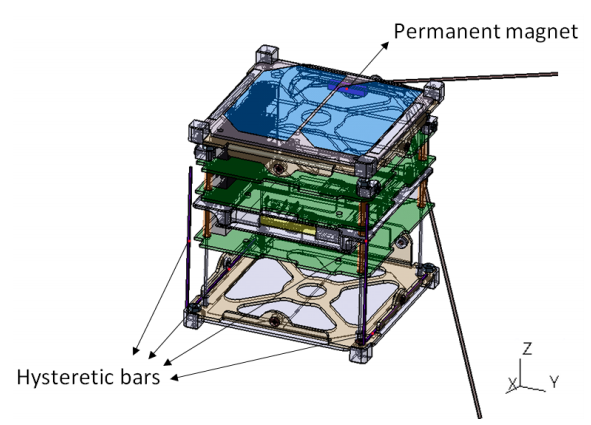
\includegraphics[scale=0.8]{1.png}
\end{center}
\end{document}